\documentclass[11pt,a4paper]{article}

% ---------------------------------------------------------------- packages
\usepackage[T1]{fontenc}
\usepackage[utf8]{inputenc}
\usepackage{lmodern}
\usepackage[margin=2.2cm,headheight=14pt]{geometry}
\usepackage{microtype}
\usepackage{graphicx}
\usepackage{booktabs}
\usepackage{tabularx}
\usepackage{array}
\usepackage[table]{xcolor}
\usepackage{enumitem}
\usepackage{caption}
\usepackage{subcaption}
\usepackage{float}
\usepackage{multicol}
\usepackage{fancyhdr}
\usepackage{titlesec}
\usepackage{tikz}
\usetikzlibrary{positioning,arrows.meta,calc,fit,backgrounds}
\usepackage[most]{tcolorbox}
\usepackage{xurl}
\usepackage[hidelinks]{hyperref}

\graphicspath{{figures/}}

% ---------------------------------------------------------------- look
\definecolor{accent}{HTML}{2F4FB8}
\definecolor{soft}{HTML}{EEF2FE}
\definecolor{ink}{HTML}{1C2230}
\definecolor{muted}{HTML}{5B6476}
\definecolor{g1}{HTML}{1F4E8C}
\definecolor{g2}{HTML}{E07A1F}
\definecolor{g3}{HTML}{6D4CE0}

\titleformat{\section}{\sffamily\Large\bfseries\color{ink}}{\color{accent}\thesection}{0.6em}{}
\titleformat{\subsection}{\sffamily\large\bfseries\color{ink}}{\color{accent}\thesubsection}{0.5em}{}
\titlespacing*{\section}{0pt}{14pt}{6pt}
\titlespacing*{\subsection}{0pt}{10pt}{4pt}

\captionsetup{font=small,labelfont={bf,sf,color=accent},skip=4pt}
\captionsetup[sub]{font=footnotesize}
\setlist{itemsep=2pt,topsep=3pt,leftmargin=*}
\setlength{\parindent}{0pt}
\setlength{\parskip}{5pt}
\renewcommand{\arraystretch}{1.25}
\newcolumntype{L}{>{\raggedright\arraybackslash}X}

\pagestyle{fancy}
\fancyhf{}
\fancyhead[L]{\sffamily\small\color{muted}Emotion-Adaptive Menus \textbar{} Phase 1 Trial Platform}
\fancyhead[R]{\sffamily\small\color{muted}\thepage}
\renewcommand{\headrulewidth}{0.4pt}

\newtcolorbox{keybox}[1][]{enhanced,colback=soft,colframe=accent,boxrule=0.6pt,arc=2mm,
  left=3mm,right=3mm,top=2mm,bottom=2mm,fonttitle=\sffamily\bfseries,title=#1}
\newcommand{\cmd}[1]{\texttt{\small #1}}
% screenshot: thin frame, never wider than the column, optional max height
\newcommand{\shot}[2][\maxdimen]{\begingroup\setlength{\fboxsep}{0pt}\setlength{\fboxrule}{0.4pt}%
  \centering\fcolorbox{black!18}{white}{\includegraphics[width=\dimexpr\linewidth-0.8pt\relax,height=#1,keepaspectratio]{#2}}\par\endgroup}

% ================================================================ document
\begin{document}

% ---------------------------------------------------------------- title block
\begin{center}
  {\sffamily\small\color{accent}\textbf{HCI PROJECT \textbullet{} LLM-BASED, EMOTION-ADAPTIVE MENUS}}\\[6pt]
  {\sffamily\huge\bfseries\color{ink} Experimental Trial Platform}\\[4pt]
  {\sffamily\large\color{muted} Phase 1: emotion-labelled data collection}\\[10pt]
  {\small [Group members] \quad\textbullet\quad Prepared for [Instructor name] \quad\textbullet\quad \today}
\end{center}
\vspace{4pt}

\begin{keybox}[At a glance]
We have built a complete, automated platform for running our trials. With a single command, it
\textbf{induces an emotion}, has the participant \textbf{complete navigation tasks on a website}, records
\textbf{eye tracking, GSR, heart rate and behaviour} on one shared clock, and saves everything as
\textbf{model-ready, labelled data}.

\smallskip
\begin{tabularx}{\linewidth}{@{}LLL@{}}
\textbf{3} groups, \textbf{6} emotions & \textbf{3} purpose-built websites & \textbf{72} matched tasks\\
$\approx$\textbf{40 min} per participant & \textbf{1 command} per session & \textbf{10} output files per participant
\end{tabularx}
\end{keybox}

% ================================================================ 1
\section{Study design}

Each group has two contrasting emotions and its own website. Every participant experiences
\textbf{both} emotions of their group (a within-subjects design), so each person serves as their own
baseline. This matters for a sample of 5--6 participants per group.

\begin{table}[H]
\centering\small
\begin{tabularx}{\linewidth}{@{}l l L L@{}}
\toprule
\textbf{Group} & \textbf{Emotions} & \textbf{Contrast in the signals} & \textbf{Website (our own build)}\\
\midrule
\textcolor{g1}{\textbf{G1}} & Stress vs.\ Calm & high vs.\ low arousal, negative vs.\ positive & University student portal\\
\textcolor{g2}{\textbf{G2}} & Frustration vs.\ Boredom & high vs.\ low arousal & Online store\\
\textcolor{g3}{\textbf{G3}} & Joy vs.\ Sadness & positive vs.\ negative valence & Discussion forum\\
\bottomrule
\end{tabularx}
\caption{Groups, emotions and websites. Each group's two emotions were chosen so they are reliable to induce in a lab and clearly separable in the physiological signals.}
\end{table}

\textbf{Counterbalancing.} The participant number decides the order of the two emotions and of the two
task sets (A/B), following a $2\times2$ Latin square, so every four consecutive participants are fully balanced.
In this phase every participant uses one \textbf{standard drop-down menu}: we collect clean
emotion-labelled data first, and build the adaptive menus from the trained model in phase 2.

% ================================================================ 2
\section{Session procedure}

The session runs on its own. The participant follows on-screen instructions and the researcher only watches.

\begin{figure}[H]
\centering
\resizebox{\linewidth}{!}{%
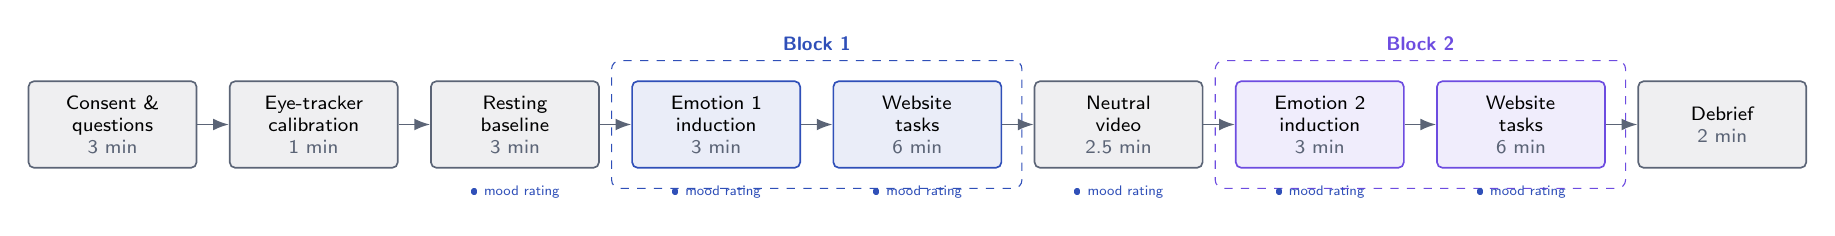
\begin{tikzpicture}[
  box/.style={draw=#1,fill=#1!10,rounded corners=2pt,minimum height=11mm,text width=19mm,align=center,font=\sffamily\scriptsize,line width=0.6pt},
  box/.default=accent,
  arr/.style={-{Latex[length=2mm]},line width=0.6pt,color=muted}]
  \node[box=muted] (c) {Consent \&\\questions\\\textcolor{muted}{3 min}};
  \node[box=muted,right=4mm of c] (k) {Eye-tracker\\calibration\\\textcolor{muted}{1 min}};
  \node[box=muted,right=4mm of k] (b) {Resting\\baseline\\\textcolor{muted}{3 min}};
  \node[box=accent,right=4mm of b] (i1) {Emotion 1\\induction\\\textcolor{muted}{3 min}};
  \node[box=accent,right=4mm of i1] (t1) {Website\\tasks\\\textcolor{muted}{6 min}};
  \node[box=muted,right=4mm of t1] (w) {Neutral\\video\\\textcolor{muted}{2.5 min}};
  \node[box=g3,right=4mm of w] (i2) {Emotion 2\\induction\\\textcolor{muted}{3 min}};
  \node[box=g3,right=4mm of i2] (t2) {Website\\tasks\\\textcolor{muted}{6 min}};
  \node[box=muted,right=4mm of t2] (d) {Debrief\\\textcolor{muted}{2 min}};
  \foreach \a/\b in {c/k,k/b,b/i1,i1/t1,t1/w,w/i2,i2/t2,t2/d} \draw[arr] (\a) -- (\b);
  \foreach \n in {b,i1,t1,w,i2,t2}
    \node[font=\sffamily\tiny,color=accent,below=1mm of \n] {\textbullet{} mood rating};
  \begin{scope}[on background layer]
    \node[draw=accent,dashed,rounded corners=3pt,fit=(i1)(t1),inner sep=2.5mm,
          label={[font=\sffamily\scriptsize\bfseries,color=accent]above:Block 1}] {};
    \node[draw=g3,dashed,rounded corners=3pt,fit=(i2)(t2),inner sep=2.5mm,
          label={[font=\sffamily\scriptsize\bfseries,color=g3]above:Block 2}] {};
  \end{scope}
\end{tikzpicture}}
\caption{One session ($\approx$40 minutes). A mood rating follows the baseline, every induction, every task block and the neutral video. Task blocks also end with a workload rating (NASA-TLX).}
\end{figure}

% ================================================================ 3
\section{Emotion induction}

Each emotion is induced with a published method \emph{before} the task block. Where the literature supports
it, a manipulation \emph{during} the tasks keeps the state going, because film clips alone fade within minutes~\cite{westermann1996}.

\begin{table}[H]
\centering\small
\begin{tabularx}{\linewidth}{@{}l L L l@{}}
\toprule
\textbf{Emotion} & \textbf{Before the tasks ($\approx$3 min)} & \textbf{During the tasks} & \textbf{Basis}\\
\midrule
Stress & Timed mental arithmetic (MIST), with a rigged ``you vs.\ average'' bar and negative feedback & Visible countdown, ``compared with other participants'' banner & \cite{dedovic2005,kirschbaum1993}\\
Calm & Nature video with paced breathing (6 breaths/min) & ``No rush'' instructions, no timer & \cite{ulrich1991,lehrer2014}\\
Frustration & Goal and incentive framing (``fastest participants get a bonus'') & Deliberate faults: slow pages, ignored clicks, menus closing, ``session expired'' & \cite{scheirer2002,ceaparu2004}\\
Boredom & Copying dull technical text & Every task uses the same repetitive template & \cite{vantilburg2012,markey2014}\\
Joy & Wordless comedy clip (\emph{Mr.\ Bean}, ``The Exam'') & Surprise ``Bonus unlocked!'' rewards & \cite{gross1995,isen1972}\\
Sadness & Sad film scene (\emph{Taare Zameen Par}), then quiet reflection & None & \cite{gross1995}\\
\bottomrule
\end{tabularx}
\caption{Induction methods. The film clips follow Gross and Levenson's method~\cite{gross1995}, but use culturally familiar clips. All inductions are checked with the participant's own mood ratings.}
\end{table}

\begin{figure}[H]
\centering
\begin{subfigure}[t]{0.32\linewidth}\shot[3.1cm]{mist.png}\caption{Stress: MIST arithmetic}\end{subfigure}\hfill
\begin{subfigure}[t]{0.32\linewidth}\shot[3.1cm]{breathing.jpg}\caption{Calm: nature and breathing}\end{subfigure}\hfill
\begin{subfigure}[t]{0.32\linewidth}\shot[3.1cm]{copying.png}\caption{Boredom: copying task}\end{subfigure}\\[6pt]
\begin{subfigure}[t]{0.32\linewidth}\shot[3.1cm]{briefing.png}\caption{Frustration: speed-bonus framing}\end{subfigure}\hfill
\begin{subfigure}[t]{0.32\linewidth}\shot[3.1cm]{film.png}\caption{Joy and sadness: film clip}\end{subfigure}\hfill
\begin{subfigure}[t]{0.32\linewidth}\shot[3.1cm]{neutral.png}\caption{Neutral video between blocks}\end{subfigure}
\caption{Induction screens as the participant sees them.}
\end{figure}

% ================================================================ 4
\section{Websites and tasks}

The three websites are our own builds on one shared engine, so menu behaviour, timing and logging are identical
across groups. Their structure is modelled on the realistic sites of the WebArena benchmark~\cite{zhou2024}:
\textbf{6 sections $\times$ 6 pages}, with the \textbf{drop-down menu as the only way to navigate}. Every page change in
the data is therefore a menu interaction, which is exactly what phase 2 will adapt.

\begin{figure}[H]
\centering
\begin{subfigure}[t]{0.32\linewidth}\shot[\maxdimen]{site_portal.png}\caption{G1: student portal}\end{subfigure}\hfill
\begin{subfigure}[t]{0.32\linewidth}\shot[\maxdimen]{site_store.png}\caption{G2: online store}\end{subfigure}\hfill
\begin{subfigure}[t]{0.32\linewidth}\shot[\maxdimen]{site_forum.png}\caption{G3: discussion forum}\end{subfigure}
\caption{The three websites (fictional brands, no internet needed).}
\end{figure}

\begin{table}[H]
\centering\small
\begin{tabularx}{\linewidth}{@{}l L L@{}}
\toprule
\textbf{Task type} & \textbf{Example (G2 store)} & \textbf{What it measures}\\
\midrule
Look-up (8 per set) & ``Find the Trailblazer 2-Person Tent. What is its price?'' & Finding the right menu path from an item name\\
Extreme (2 per set) & ``Find the cheapest vitamin or supplement.'' & Navigating, then scanning a page\\
Compare (2 per set) & ``Which is cheaper: the Yoga Mat or the Vitamin C Serum?'' & Navigating across several pages\\
\bottomrule
\end{tabularx}
\caption{Each website has two matched task sets (A and B) of 12 tasks. Answers are multiple choice and are computed automatically from the site content.}
\end{table}

Each task block lasts exactly \textbf{6 minutes}, so every emotion yields the same amount of data per person.

\begin{figure}[H]
\centering
\begin{subfigure}[t]{0.49\linewidth}\shot[\maxdimen]{task_stress.png}\caption{Stress: countdown, recording banner, answer panel and feedback}\end{subfigure}\hfill
\begin{subfigure}[t]{0.49\linewidth}\shot[\maxdimen]{task_frustration.png}\caption{Frustration: page loading lag and a fake ``session expired'' error}\end{subfigure}\\[6pt]
\begin{subfigure}[t]{0.49\linewidth}\shot[\maxdimen]{task_joy.png}\caption{Joy: surprise bonus reward}\end{subfigure}\hfill
\begin{subfigure}[t]{0.49\linewidth}\shot[\maxdimen]{task_menu.png}\caption{The standard drop-down menu in use}\end{subfigure}
\caption{The task screen: the task bar sits above the live website.}
\end{figure}

% ================================================================ 5
\section{Measures and data}

\begin{table}[H]
\centering\small
\begin{tabularx}{\linewidth}{@{}l L@{}}
\toprule
\textbf{Source} & \textbf{What is recorded}\\
\midrule
Eye tracker (Tobii Pro) & Gaze position and pupil size (60--120 Hz), mapped to menu items and page content\\
GSR & Skin conductance in microsiemens (supports Shimmer3, LSL devices, Arduino)\\
Heart rate & BPM and RR intervals (supports Polar H10, LSL, serial)\\
Behaviour & Every click, menu open/hover/close, page view, mouse movement (60 Hz), task outcome and time\\
Self-report & SAM valence/arousal/dominance~\cite{bradley1994}, six emotion ratings, NASA-TLX~\cite{hart1988}\\
\bottomrule
\end{tabularx}
\caption{Measures. All streams share one master clock; the eye tracker's clock offset is re-measured every 30 s.}
\end{table}

Each participant gets one folder, for example \cmd{data/G2/P04/}, containing the raw streams (gaze, GSR, heart rate,
events, mouse, tasks, questionnaires) and \textbf{\cmd{merged.csv}}: a 10 Hz timeline that combines every signal with
its phase, emotion and task labels, ready for model training. Table~\ref{tab:merged} shows an excerpt.

\begin{table}[H]
\centering\footnotesize
\begin{tabularx}{\linewidth}{@{}r l l r r r L r r@{}}
\toprule
\textbf{t (s)} & \textbf{Emotion} & \textbf{Task} & \textbf{Gaze x} & \textbf{Gaze y} & \textbf{Pupil} & \textbf{Looking at} & \textbf{GSR} & \textbf{HR}\\
\midrule
143.6 & stress & B01 & 0.496 & 0.505 & 3.89 & content: Mr Tom Reyes & 7.46 & 77\\
143.7 & stress & B01 & 0.494 & 0.499 & 3.90 & content: Mr Tom Reyes & 7.44 & 77\\
143.8 & stress & B01 & 0.499 & 0.489 & 3.86 & content: Dr Helen Moore & 7.42 & 77\\
\bottomrule
\end{tabularx}
\caption{Excerpt of \texttt{merged.csv} from a dry run with simulated sensors (selected columns).}
\label{tab:merged}
\end{table}

% ================================================================ 6
\section{Running a session}

\begin{keybox}[Researcher workflow]
\begin{tabularx}{\linewidth}{@{}l L@{}}
\cmd{python run.py check} & Checks sensors, videos, browser and task answers; must say ``Ready.''\\
\cmd{python run.py session -{}-group G2 -{}-participant P04} & Runs the full session in a fullscreen browser\\
\cmd{python run.py export} & Combines all participants into one dataset\\
\end{tabularx}
\end{keybox}

\begin{figure}[H]
\centering
\begin{minipage}{0.82\linewidth}\shot{console.png}\end{minipage}
\caption{The researcher's live terminal view during a session: current phase, emotion, task and sensor health. The participant never sees it.}
\end{figure}

Built-in safeguards:
\begin{itemize}
  \item A session will not start if a sensor sends no data or a video is missing.
  \item Every data row is saved immediately, and an interrupted session can be resumed.
  \item A participant ID can never be reused by accident.
  \item Participants never see emotion names or correct answers.
\end{itemize}

% ================================================================ 7
\section{Ethics}

\begin{itemize}
  \item Participants sign a consent form that says, in general terms, that some activities are designed to influence how they feel.
  \item The on-screen debrief then explains exactly which manipulations they experienced (for example, that the website lag was deliberate) and asks again for permission to use their data.
  \item If the participant declines, at the start or at the debrief, \textbf{their data is deleted automatically}.
  \item Inductions are brief and mild, and the researcher gives a verbal wellbeing check at the end.
\end{itemize}

% ================================================================ 8
\section{Status and next steps}

\begin{table}[H]
\centering\small\renewcommand{\arraystretch}{1.1}
\begin{tabularx}{\linewidth}{@{}L l@{}}
\toprule
\textbf{Item} & \textbf{Status}\\
\midrule
Websites, tasks, inductions, questionnaires, debrief (all three groups) & \textcolor{g1}{\textbf{Done}}\\
Videos (nature, neutral, amusement, sadness) & \textcolor{g1}{\textbf{Done}}\\
Full dry runs for all groups with simulated sensors; 17 automated tests & \textcolor{g1}{\textbf{Passed}}\\
Set the GSR and heart-rate device models; one dry run on the real hardware & \textcolor{g2}{\textbf{Next}}\\
Ethics approval; recruit 5--6 participants per group (15--18 in total) & \textcolor{g2}{\textbf{Next}}\\
Phase 2: train the emotion model and build the adaptive menus & \textcolor{muted}{\textbf{Later}}\\
\bottomrule
\end{tabularx}
\end{table}

% ================================================================ references
\vspace{-6pt}
\subsection*{References}
\vspace{-2pt}
\begingroup
\footnotesize
\renewcommand{\section}[2]{}
\begin{multicols}{2}
\begin{thebibliography}{99}\setlength{\itemsep}{0pt}
\bibitem{bradley1994} M.~M. Bradley and P.~J. Lang. Measuring emotion: The Self-Assessment Manikin and the semantic differential. \emph{J.\ Behav.\ Ther.\ Exp.\ Psychiatry}, 25(1):49--59, 1994.
\bibitem{ceaparu2004} I.~Ceaparu, J.~Lazar, K.~Bessiere, J.~Robinson, and B.~Shneiderman. Determining causes and severity of end-user frustration. \emph{Int.\ J.\ Human-Computer Interaction}, 17(3):333--356, 2004.
\bibitem{dedovic2005} K.~Dedovic et al. The Montreal Imaging Stress Task. \emph{J.\ Psychiatry \& Neuroscience}, 30(5):319--325, 2005.
\bibitem{gross1995} J.~J. Gross and R.~W. Levenson. Emotion elicitation using films. \emph{Cognition and Emotion}, 9(1):87--108, 1995.
\bibitem{hart1988} S.~G. Hart and L.~E. Staveland. Development of NASA-TLX. \emph{Advances in Psychology}, 52:139--183, 1988.
\bibitem{isen1972} A.~M. Isen and P.~F. Levin. Effect of feeling good on helping: Cookies and kindness. \emph{J.\ Pers.\ Soc.\ Psychology}, 21(3):384--388, 1972.
\bibitem{kirschbaum1993} C.~Kirschbaum, K.~M. Pirke, and D.~H. Hellhammer. The ``Trier Social Stress Test''. \emph{Neuropsychobiology}, 28(1--2):76--81, 1993.
\bibitem{lehrer2014} P.~M. Lehrer and R.~Gevirtz. Heart rate variability biofeedback: How and why does it work? \emph{Frontiers in Psychology}, 5:756, 2014.
\bibitem{markey2014} A.~Markey, A.~Chin, E.~M. Vanepps, and G.~Loewenstein. Identifying a reliable boredom induction. \emph{Perceptual and Motor Skills}, 119(1):237--253, 2014.
\bibitem{scheirer2002} J.~Scheirer, R.~Fernandez, J.~Klein, and R.~W. Picard. Frustrating the user on purpose. \emph{Interacting with Computers}, 14(2):93--118, 2002.
\bibitem{ulrich1991} R.~S. Ulrich et al. Stress recovery during exposure to natural and urban environments. \emph{J.\ Environmental Psychology}, 11(3):201--230, 1991.
\bibitem{vantilburg2012} W.~A.~P. van Tilburg and E.~R. Igou. On boredom: Lack of challenge and meaning as distinct boredom experiences. \emph{Motivation and Emotion}, 36(2):181--194, 2012.
\bibitem{westermann1996} R.~Westermann, K.~Spies, G.~Stahl, and F.~W. Hesse. Relative effectiveness and validity of mood induction procedures: A meta-analysis. \emph{European J.\ Social Psychology}, 26(4):557--580, 1996.
\bibitem{zhou2024} S.~Zhou et al. WebArena: A realistic web environment for building autonomous agents. In \emph{Proc.\ ICLR}, 2024.
\end{thebibliography}
\end{multicols}
\endgroup

% ================================================================ appendix
\clearpage
\appendix
\section{Participant screens}

\begin{figure}[H]
\centering
\begin{subfigure}[t]{0.49\linewidth}\shot[4.5cm]{welcome.png}\caption{Welcome}\end{subfigure}\hfill
\begin{subfigure}[t]{0.49\linewidth}\shot[4.5cm]{consent.png}\caption{On-screen consent}\end{subfigure}\\[6pt]
\begin{subfigure}[t]{0.49\linewidth}\shot[4.5cm]{calibration.png}\caption{Eye-tracker calibration}\end{subfigure}\hfill
\begin{subfigure}[t]{0.49\linewidth}\shot[4.5cm]{rest.png}\caption{Resting baseline (fixation cross)}\end{subfigure}\\[6pt]
\begin{subfigure}[t]{0.49\linewidth}\shot[4.5cm]{sam.png}\caption{Mood rating: Self-Assessment Manikin}\end{subfigure}\hfill
\begin{subfigure}[t]{0.49\linewidth}\shot[4.5cm]{emotions.png}\caption{Mood rating: six emotions (order shuffled)}\end{subfigure}\\[6pt]
\begin{subfigure}[t]{0.49\linewidth}\shot[4.5cm]{tlx.png}\caption{Workload rating (NASA-TLX)}\end{subfigure}\hfill
\begin{subfigure}[t]{0.49\linewidth}\shot[4.5cm]{debrief.png}\caption{Debrief, with the option to withdraw}\end{subfigure}
\caption{The remaining screens of a session.}
\end{figure}

\end{document}
